\section{UES - Join Ordering with Simple Upper Bound}
\label{sec:UES}

In contrast to state-of-the-art approaches, our \emph{UES} concept~\cite{hertzschuch-21-ues} follows a completely different idea to determine good join orderings for SPJ queries: it calculates theoretical upper bounds of the sizes of intermediate result sets and uses these bounds in a heuristic join enumeration algorithm. 
This concept is based on the insight that the duration of query workloads is often dominated by the runtime of very few queries which take an exceptionally long amount of time. 
Meanwhile, most queries in a typical workload can be answered rather quickly. 
This phenomena is referred to as \emph{tail latency}.
Thus, a novel query optimization strategy should focus on improving these long queries, instead of speeding up queries that are already fast. 
However, this can usually not be achieved by improving the runtime in the average case, since new outliers can become part of the tail latencies. 
In contrast, a correct theoretical upper bound can never be wrong in the sense that the true cardinalities exceed the bound. 
By feeding these worst-case estimates to the join enumeration algorithm, it will probably choose a join order that is too pessimistic in the sense that another join order could have provided a faster runtime. 
But it will never choose a join order that is too optimistic, i.e. a plan that only works if the intermediate cardinalities are indeed small and takes a much longer time to execute if this hope is not met.

%In practice, the plan of a pessimistic optimization algorithm could still introduce regressions. 
%But these regressions are caused by errors in the cost model, rather than the estimates. 
%And such cost model regressions also exist in more optimistic estimation and enumeration strategies.
%By choosing plans that are more defensive than necessary, the runtime of many fast queries might increase slightly. 
%Following the mindset of the UES algorithm, this is acceptable as long as the tail latencies can be reduced substantially. 
%To justify the focus on tail latencies, consider once again the Join Order Benchmark~\cite{DBLP:journals/pvldb/LeisGMBK015}. Figure~\ref{fig:JOBRuntimes}(a) shows the execution time of each query in the workload. 
%The ten longest-running queries amount to over 50\% of the total workload runtime. 
%If the runtime of these queries can be reduced, e.g., by using the UES algorithm (cf. Figure~\ref{fig:jobJOBRuntimes}(b)), the ten longest-running queries only amount to about 20\% of the total runtime (which is also partly due to an increased runtime of other queries).

%\begin{figure}[t]
%    \centering
%    \begin{tabular}{cc}
%    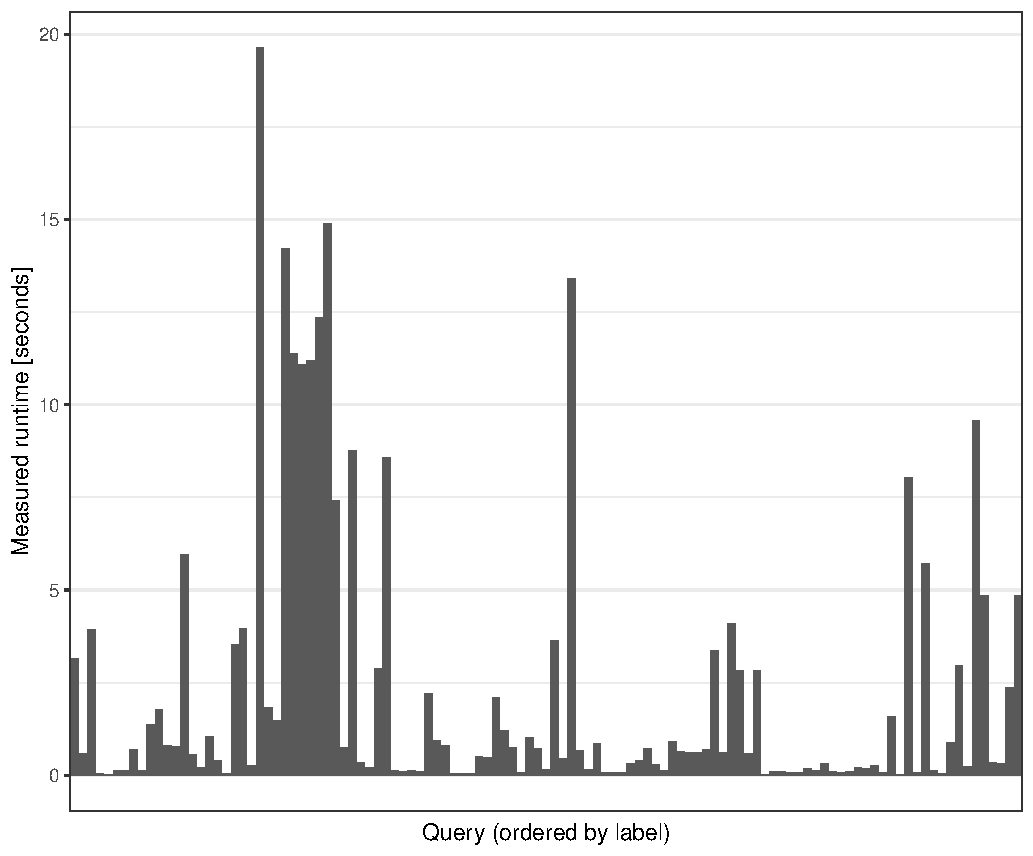
\includegraphics[width=0.47\linewidth]{figures/plot-job-implicit.pdf}
%    & \includegraphics[width=0.47\linewidth]{figures/plot-job-ues.pdf} \\
%    (a) Optimized by PostgreSQL &
%   (b) Optimized by UES 
%    \end{tabular}
%    \caption{JOB query runtimes. Each query is repeated 5 times, with the best runtime being depicted.}
%    \label{fig:JOBRuntimes}
%    \vspace{-0.4cm}
%\end{figure}



Our \emph{UES} upper bounds of join intermediate cardinalities are estimated via most frequent value statistics on the join columns. 
For brevity the calculation is only summarized here, since the final formula is already presented and justified in~\cite{hertzschuch-21-ues}.
To estimate the size of a join $R.x \bowtie S.y$ on (filtered) base tables $R$ and $S$ based only on the most frequent values for $R.x$ and $S.y$, a first pessimistic assumption is used: the attributes are \emph{assumed} to be uniformly distributed, with the maximum value frequency (MF) therefore also being the only frequency shared by all values. 
Based on these frequencies and the total number of tuples per (filtered) relation ($|\sigma(R.x)|, |\sigma(S.y)|$), the minimum number of distinct values per attribute can also be estimated.
To combine these per-table values into an estimate for their join result, a second pessimistic assumption is used: the attribute values are assumed to overlap perfectly, i.e. each value in $R.x$ has a matching join partner in $S.y$. 
This leads to $MF(R.x) * MF(S.y)$ many outgoing tuples per value combination. 
Since there are at most $min(|\sigma(R.x)| / MF(R.x), |\sigma(S.y)| / MF(S.y))$ many such combinations, the upper bound can be calculated as
$$upper(|\sigma(R) \bowtie \sigma(S)|) := min\Bigl(\frac{|\sigma(R)|}{MF(R.x)}, \frac{|\sigma(S)|}{MF(S.y)}\Bigr) * MF(R.x) * MF(S.y)$$

\begin{figure}[t]
    \centering
    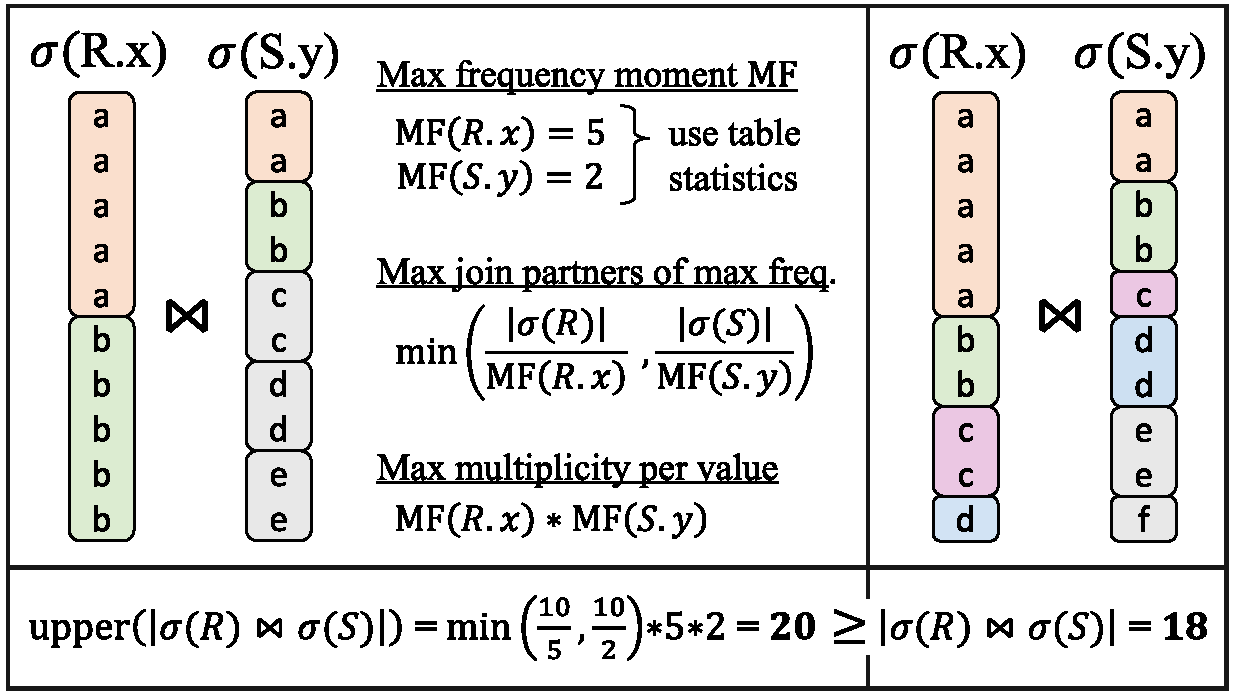
\includegraphics[width=0.7\linewidth]{figures/upperBoundExplV6_.pdf}
    \caption{Illustration of the UES upper bound (taken from \cite{hertzschuch-21-ues}).}
    \label{fig:upperBoundExpl}
    \vspace{-0.4cm}
\end{figure}

Fig.~\ref{fig:upperBoundExpl} illustrates our UES upper bound concept, using an example. 
The left-hand side depicts the worst-case -- used to derive the upper bound -- constrained by the table statistics, while the right-hand side depicts the actual join.
Note that $R$ and $S$ do not need to be base tables. 
Instead they can be the result of some other join just as well. 
For example, without loss of generality, we can assume that $R = R_1 \bowtie_{R_1.a = R_2.b} R_2$. 
In this case, $|\sigma(R)| = upper(|R_1 \bowtie R_2|)$ and $MF(R.x) = MF(R_1.a) * MF(R_2.b)$. 
This enables the calculation of upper bounds for any join in a recursive manner. 
One central downside of this approach is the propagation of errors, in this case of overestimated result sizes. 
Since the estimation of an $n$-way join requires estimates of $n-1 $ smaller joins building on top of each other, estimates grow larger and larger as shown in Fig.~\ref{fig:UESOverestimationJOB}.
%This puts special emphasis on the importance of tight upper bounds. 

Based on this upper bound of join cardinalities, the join order in \emph{UES} is obtained using a heuristic algorithm~\cite{hertzschuch-21-ues}.
The UES enumeration algorithm tries to choose each join such that the sizes of intermediate results are minimized in each step. 
To make this choice, the upper bounds of candidate joins are calculated and the join with smallest bound is executed. 
However, this process is only applied to n:m joins. 
Primary key/Foreign key joins (P/K joins) are greedily included as soon as possible. 
This strategy is justified by a central property of P/K joins: When the Foreign Key partner is already present in the intermediate result, joining the Primary Key table may only reduce, but never expand the size of the intermediate result. In this sense, P/K joins act as special filters. 
To facilitate this filtering property even further, a P/K join can be executed as a subquery: suppose an (intermediate) table $\Tilde{T}$ should be joined with a Foreign Key table $T_{FK}$, which in turn has to be joined with a Primary Key table $T_{PK}$. 
The canonical way of executing this join would be $(\Tilde{T} \bowtie T_{FK}) \bowtie T_{PK}$. The n:m join $\Tilde{T} \bowtie T_{FK}$ would most likely (i.e. following the pessimistic assumption) increase the size of the intermediate result. 
Afterwards, joining $T_{PK}$ could potentially reduce the size of the intermediate result again. 
If such a reduction is guaranteed, executing $T' := T_{FK} \bowtie T_{PK}$ first and afterwards $\Tilde{T} \bowtie T'$ would minimize work for the second join. Thus, when choosing the next n:m join to execute, UES tries to pre-filter the join partners via P/K joins. 
If this does not guarantee a smaller intermediate result, the Primary Key partner will be joined after the n:m join has been executed.


%\setlength{\abovecaptionskip}{8pt plus 3pt minus 2pt}
%\begin{figure*}[t]
%    \centering
%    \subfloat[\mbox{Implicit Syntax – Joins yet to be ordered}]{\includegraphics[width=0.385\textwidth]{figures/rewriting_aV2.pdf}\label{fig:SQL_Rewriting_A}} \hspace*{0.32cm}
%    \subfloat[Explicit Join Order - Physical operators yet to be determined]{\includegraphics[width=0.58\textwidth]{figures/rewriting_bV3.pdf}\label{fig:SQL_Rewriting_B}}
%		\todo[inline]{adjust caption, it des not really relate to the pictures.}
%    \caption{Rewriting of JOB query 18a according to \textit{UES}. Non-expanding operators (pk-fk joins, filters) are highlighted green and potentially expanding operators (n:m joins) are highlighted red. } %among the two estimates.}
%    \label{fig:SQL_Rewriting}%
%\end{figure*}


%%%%%%%%%%%%
% DH: Das könnte eventuell noch ungeschrieben werden
%%%%%%%%%
%In contrast to a traditional full-fledged optimizer, UES does not choose the physical join operators to carry out each join. This task is still left to the normal optimizer. However, the available choices are restricted through database-specific options to disable Nested Loop Joins, which essentially forces Hash Joins for the largest part of a query. In the initial presentation of UES this restriction was necessary because the UES implementation did not actually replace the query optimizer. Instead, it acted as a wrapper, providing the database system with an optimized join order and forced the system to stick to that order. However, the system still had to run its own optimization process (which was now only responsible for choosing the plan operators). Since this process again involved overly optimistic intermediate size estimates via the system-specific statistics, the optimizer was prone to choose Nested Loop Joins in situations where they were not appropriate. By also restricting the choice of operators, this flaw can be mitigated. Through the extensions presented in the next chapter, specifically Section~\ref{sec:ues-extension-query-hints}, this constraint can now be lifted.
